\documentclass[12pt]{report}
\usepackage{graphicx}
\usepackage{amsmath}
\usepackage{listings}
\usepackage{color}
\usepackage[numbers]{natbib}
\usepackage{bibentry}
\usepackage{rotating}
\usepackage{float}
\usepackage[utf8]{inputenc} 
\setlength{\arrayrulewidth}{0.1mm}
\setlength{\tabcolsep}{18pt}

\renewcommand{\arraystretch}{1.5}
\usepackage[left=3cm, right=3cm, top=3cm]{geometry}
\definecolor{dkgreen}{rgb}{0,0.6,0}
\definecolor{gray}{rgb}{0.5,0.5,0.5}
\definecolor{mauve}{rgb}{0.58,0,0.82}
\lstset{frame=tb,
  language=Java,
  aboveskip=3mm,
  belowskip=3mm,
  showstringspaces=false,
  columns=flexible,
  basicstyle={\small\ttfamily},
  numbers=none,
  numberstyle=\tiny\color{gray},
  keywordstyle=\color{blue},
  commentstyle=\color{dkgreen},
  stringstyle=\color{mauve},
  breaklines=true,
  breakatwhitespace=true,
  tabsize=3
}

\usepackage{amssymb}
\setlength\parindent{0pt}

\begin{document}


\begin{center}
\begin{large}
\textbf{ Webform  Optimisation Using Machine Learning }
\end{large}
\end{center}
\vspace*{30px}
\begin{center}
A project report submitted in complete fulfillment of the requirements for the degree
\begin{center}
\hspace*{-80px}of
\end{center}
\hspace*{30px} \textbf{ Bachelor Of Engineering }
\newline
\newline
\hspace*{50px}by
\newline
\newline
\newline
\hspace*{30px} \textbf{Akshaykumar Hanmandla (Roll no 7699)}
\newline
\hspace*{30px} \textbf{Jaydeep Ranoliya (Roll no 7719)}
\newline
\hspace*{30px} \textbf{Dhananjaykumar Ojha (Roll no 7713)}
\newline
\newline
\newline
\newline
\hspace*{50px} Under the guidance of 
\newline
\hspace*{60px}\textbf{Saurabh Kulkarni}
\newline
\newline
\begin{center}
\begin{figure}[!ht]
\hspace*{125px}
\includegraphics[scale=0.3]{crcelogo.jpg}
\end{figure}
\end{center}
\end{center}
\hspace*{90px} DEPARTMENT OF INFORMATION TECHNOLOGY
\newline
\begin{center}
 Fr. Conceicao Rodrigues College of Engineering, Bandra (W), Mumbai - 400050
\newline
\newline
\hspace*{60px} \textbf{ University of Mumbai}
\newline
April 25, 2019
\end{center}
\newpage
\vspace*{230px}
\begin{center}
\hspace*{50px}
\textit{This work is dedicated to our family.}
\newline
\textit{We are very thankful for their motivation and support.}
\end{center}
\newpage
\begin{center}
\begin{Huge}
\hspace*{23px}
\textbf{ Internal Approval Sheet }
\newline
\newline
\newline
\vspace*{23px}
CERTIFICATE
\end{Huge}
\end{center}
\vspace*{80px}
This is to certify that the project entitled \textbf{Webform Optimization using Machine
Learning} is a bonafide work of \textbf{Akshaykumar Hanmandla(7699), Jaydeep Ranoliya(7719)}
and \textbf{Dhananjaykumar Ojha(7713)} submitted to the University of Mumbai in partial fulfillment of
the requirement for the award of the degree of\textbf{ Bachelor of Engineering in Information Technology}
\vspace*{60px}
\begin{center}
\hspace*{80px}
(Name and sign)
\newline
Supervisor/Guide
\end{center}
\vspace*{100px}
\hspace*{30px}
(Name and sign)
\hspace*{230px}
(Name and sign)
\vspace*{5px}
\hspace*{30px}
Head of Department
\hspace*{230px}
Principal
\newpage
\begin{center}
\begin{Huge}
\hspace*{28px}
\textbf{ Project Approval Sheet }
\newline
\newline
\newline
\vspace*{23px}
CERTIFICATE
\end{Huge}
\end{center}
\vspace*{50px}
This project report entitled by \textbf{Webform Optimization using Machine Learning} by\textbf{ Akshaykumar  Hanmandla(7699)}, \textbf{Jaydeep Ranoliya(7719)} and \textbf{Dhananjaykumar  Ojha(7713)} is approved for the degree of \textbf{Bachelor of Engineering}

\vspace*{50px}
\hspace*{280px}
Examiners
\newline
\newline
\hspace*{280px} {1.\_\_\_\_\_\_\_\_\_\_\_\_\_\_\_\_\_\_\_\_\_\_}
\newline
\newline
\hspace*{280px}
{2.\_\_\_\_\_\_\_\_\_\_\_\_\_\_\_\_\_\_\_\_\_\_}
\newline
\vspace*{50px}
\newline
Place :
\newline
Date :
\newpage
\begin{center}
\begin{Huge}
\textbf{ Declaration }
\end{Huge}
\end{center}
\vspace*{50px}
We declare that this written submission represents our ideas in our own words and where others’ ideas or words have been included, we have adequately cited and referenced the original sources. We also declare that we have adhered to all principles of academic honesty and integrity and have not misrepresented or fabricated or falsified any idea/data/fact/source in my submission. We understand that any violation of the above will be cause for disciplinary action by the Institute and can also evoke penal action from the sources which have thus not been properly cited or from whom proper permission has not been taken when needed.
\vspace*{120px}
\hspace*{240px}
\newline 
\hspace*{140px}
Akshaykumar Hanmandla (Roll No. 7699) (sign) \_\_\_\_\_\_\_\_\_\_\_
\newline 
\hspace*{140px} 
Jaydeep Ranoliya    (Roll No. 7719) (sign) 
\hspace*{40px} 
\_\_\_\_\_\_\_\_\_\_\_
\newline 
\hspace*{140px} 
 Dhananjaykumar Ojha   (Roll No.  7713) (sign) 
\hspace*{20px} 
\_\_\_\_\_\_\_\_\_\_\_
\newline
\newline
\newline
\newline
\newline
\newline
\newline
\newline
Date :-  April 25, 2019
\newpage
\begin{center}
\begin{Huge}
\textbf{ Abstract }
\end{Huge}
\end{center}
\vspace*{50px}
Forms are used in websites for improving business and user experience\cite{krug2000don}. If the form length is big, then we get more information but information is less accurate and vice versa. Nowadays, A/B testing algorithm is being used for getting the optimal web form from a number of web forms to choose. A/B test distributes the forms uniformly to the visitors. The winning form will be the form which has more no. of conversions. So, after deploying new version of form, A/B test explores all the forms equally\cite{cruz2018enabling}. Even though some forms do not perform well, it still explores which is wastage of time and resources. So, there is more time given for exploration in A/B test. And also owner of website during testing period focuses more on testing than running the website, due to which there may be a loss of visitors. 
To overcome this problem, we can use some automated machine learning algorithms to predict the optimal web form from a number of forms to choose. These algorithms does not waste time and resources exploring inferior forms due to which we will get the results in less time and also we can simultaneously run the website.

\newpage
\begin{center}
\begin{Huge}
\textbf{ Acknowledgements }
\end{Huge}
\end{center}
\vspace*{50px}
We have great pleasure in presenting the report on \textbf{'Webform Optimization using Machine learning'}. We take this opportunity to express our sincere thanks towards the guide \textbf{Mr.Saurabh Kulkarni}, C.R.C.E, Bandra (W), Mumbai, for providing the technical guidelines, and the suggestions regarding the line of this work. We enjoyed discussing the work progress with him during our visits to department.
\newline
\newline
We thank \textbf{Mrs.Garima Tripathi}, Head of Information Technology Dept., Principal and the management of C.R.C.E., Mumbai for encouragement and providing necessary infrastructure for pursuing the project.
\newline
\newline
We also thank all non-teaching staff for their valuable support, to complete our project.
\vspace*{100px}
\hspace*{240px}
\newline 
\hspace*{160px}
Akshaykumar Hanmandla (Roll No. 7699) (sign) \_\_\_\_\_\_\_\_\_\_\_\_\_\_\_\_
\newline 
\hspace*{160px} 
Jaydeep Ranoliya    (Roll No. 7719) (sign) 
\hspace*{40px} 
\_\_\_\_\_\_\_\_\_\_\_\_\_\_\_\_
\newline 
\hspace*{160px} 
 Dhananjaykumar Ojha   (Roll No.  7713) (sign) 
\hspace*{11px} 
\_\_\_\_\_\_\_\_\_\_\_\_\_\_\_\_\_
\newpage
\tableofcontents
\listoffigures
\vspace*{10px}
\textbf{ References }
\hspace*{360px}21
\newpage
\chapter{Introduction}
\section{Background}
The use of websites is increasing day by day. By considering the past trends, the use of websites has increased exponentially from the last decade. Websites are used for running the businesses online, forums, social media sites, etc. Forms are used in websites for improving business and user experience as well as for various purposes. The owners of website get feedback from the form and accordingly they can adjust their services. Most of the users coming to the websites don’t fill the form due to lack of interest and owner of website don’t get appropriate feedback. There are many solutions to overcome this problem. The most familiar solution is A/B testing.
\section{
Motivation}
Nowadays, there are more websites coming into the online market. Forms play a major role in improving conversions of a websites. There may be a situation that user may not like to fill the form which causes loss of conversions\cite{nielsen1994usability}. To overcome this problem, we have to choose the best form so that most users will fill the form. In choosing the best version of a form on a page, most people use A/B testing. But it discretely jumps from exploration to exploitation. And, it gives equal chance to the inferior forms which do not perform well which leads into wastage of time and resources.\cite{lattimore2018bandit}
This is the area our project wants to work into: selecting the best form to put into a website so that more users will fill. And to develop an algorithm gives the best form in less time and efficient way than A/B testing.
\newpage
\section{Overview}
In this experiment, we are comparing two algorithms for selection of best form out of no. of forms to choose. 
\subsection{A/B test}
This algorithm distributes the available forms uniformly to the visitors visiting the website. This method has been found effective in various testing environments. Most of the people use this type of test to test whether the change in any website would be good or bad. The same technique we are applying for selecting the best form\cite{white2012bandit}. 

\subsection{Adaptive Epsilon Greedy}
An initial epsilon value has to be set. As the algorithm starts running, the epsilon value adjusts automatically (increases or decreases) according to the responses given by the user. Fully automated testing. Algorithms behaves according to the previous experiences learnt while in A/B test behaves the same in all the conditions\cite{white2012bandit}.
\newline
At the end, we compare the performance of both the algorithms.

\section{Scope}
We have implemented an algorithm which selects the best and optimal form in an efficient way. It learns by itself and It explores as well as exploits (Earn while you learn). We have experimented for three forms and it can be done for n number of forms.  It shows best possible version while it exploits rather than showing bad version which does not perform well. It can be implemented for other elements of websites like logo, banner, background colour, navigation bar, etc. This algorithm can be extended for entire web page or website also.  



\newpage
\chapter{Literature Review}
\section{Enabling Adaptability in Web Forms Based on User Characteristics Detection Through A/B Testing and Machine Learning}
This paper presents an original study with the aim of improving users' performance in completing large questionnaires through adaptability in web forms. Such adaptability is based on the application of machine-learning procedures and an A/B testing approach. To detect the user preferences, behavior, and the optimal version of the forms for all kinds of users, researchers built predictive models using machine-learning algorithms (trained with data from more than 3000 users who participated previously in the questionnaires), extracting the most relevant factors that describe the models, and clustering the users based on their similar characteristics and these factors. Based on these groups and their performance in the system, the researchers generated heuristic rules between the different versions of the web forms to guide users to the most adequate version (modifying the user interface and user experience) for them. To validate the approach and confirm the improvements, the authors tested these redirection rules on a group of more than 1000 users. The results with this cohort of users were better than those achieved without redirection rules at the initial stage. Besides these promising results, the paper proposes a future study that would enhance the process (or automate it) as well as push its application to other fields
\cite{cruz2018enabling}.
\newpage
\section{Online Controlled Experiments and A/B Testing}
The Internet connectivity of client software (e.g., apps running on phones and PCs), websites, and online services provide an unprecedented opportunity to evaluate ideas quickly using controlled experiments, also called A/B tests, split tests, randomized experiments, control/treatment tests, and online field experiments. Unlike most data mining techniques for finding correlational patterns, controlled experiments allow establishing a causal relationship with high probability. Experimenters can utilize the scientific method to form a hypothesis of the form “If a specific change is introduced, will it improve key metrics?” and evaluate it with real users. The theory of a controlled experiment dates back to Sir Ronald A. Fisher’s experiments at the Rothamsted Agricultural Experimental Station in England in the 1920s, and the topic of offline experiments is well developed in Statistics (Box et al., Statistics for experimenters: design, innovation, and discovery. Wiley, Hoboken, 2005). Online-controlled experiments started to be used in the late 1990s with the growth of the Internet. Today, many large sites, including Amazon, Bing, Facebook, Google, LinkedIn, and Yahoo!, run thousands to tens of thousands of experiments each year testing user interface (UI) changes, enhancements to algorithms (search, ads, personalization, recommendation, etc.), changes to apps, content management system, etc. Online-controlled experiments are now considered an indispensable tool, and their use is growing for startups and smaller websites. Controlled experiments are especially useful in combination with Agile software development (Martin, Clean code: a handbook of Agile software craftsmanship. Prentice Hall, Upper Saddle River, 2008; Rubin, Essential scrum: a practical guide to the most popular Agile process. Addison-Wesley Professional, Upper Saddle River, 2012), Steve Blank’s Customer Development process (Blank, The four steps to the epiphany: successful strategies for products that win. Cafepress.com., 2005), and MVPs (minimum viable products) popularized by Eric Ries’s Lean Startup (Ries, The lean startup: how today’s entrepreneurs use continuous innovation to create radically successful businesses. Crown Business, New York, 2011)\cite{kohavi2017online}.
\chapter{Problem Description}
\section{Problem Statement}
Forms are used in websites for signup and getting feedback from users. Sometimes, there may be a problem if owner wants to add new fields to the form because customers may feel difficult which in turn affect business.To develop a system which will help the business to not go into loss while testing the website forms. Owners can earn while learning. The strategy used in the website for testing the users will not affect the ROI (Return On Investment ) as in A/B testing\cite{seckler2015trust}. Implicit indirect feedback will be taken from visitors (without knowing them) for new web forms. Gives results to owner regarding changes in a particular website form will actually attract the visitors or reduce the number of visitors. So, we implemented an algorithm which gives an optimal web form from a no. of web forms to choose.
\newpage
\section{Data flow diagram}
A data flow diagram gives the basic idea of the flow of data in an information system while giving a short overview of its processing steps.
\subsection{DFD Level 0}
\begin{figure}[!ht]
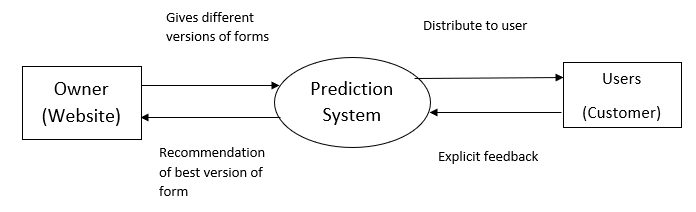
\includegraphics[scale=0.7,height=5cm,width=16.5cm]{dfd0.png}
\caption{DFD level 0}
\end{figure}
At DFD Level 0 there are 2 entities which are, Website and the User. The website provides the form which user fills. The filled information is sent to the Prediction System which gives optimal of the form for a website.
\newpage
\subsection{DFD Level 1}
\begin{figure}[!ht]
\hspace*{-30px}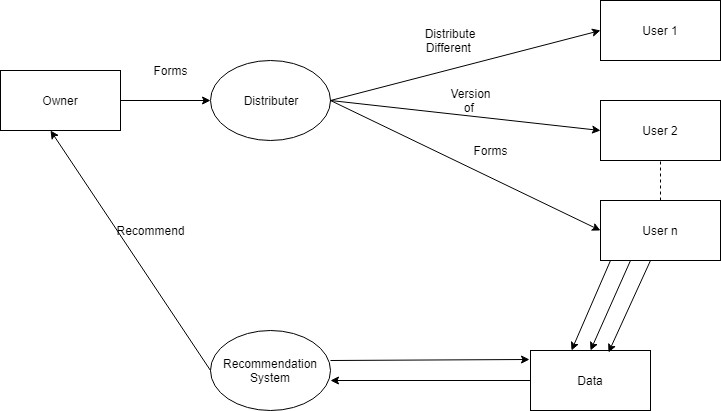
\includegraphics[scale=0.7,width=16cm,height=10cm]{dfd1.jpg}
\caption{DFD level 1}
\end{figure}
At DFD Level 1, the website gives the forms to the algorithm. The algorithm distributes the forms to the users based on some probability.Then, user fills the form. The user's characteristics of filling the form is stored in the database. The prediction system uses the data in the database and provides the optimal webform to the website owner.
\newpage
\section{Design}
\hspace*{-100px} \begin{figure}[!ht]
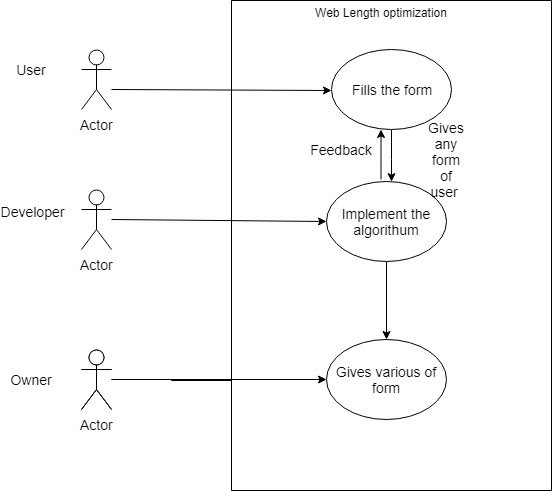
\includegraphics[scale=0.7,height=8cm,width=10.5cm]{usecase.png}
\caption{Usecase Diagram}
\end{figure}
\newline
In the above use case diagram, there are three actors 1) User 2) Developer 3) Owner. Owner gives various forms. Developer wirtes the algorithm and integrates it with the form.User fills the form from which input is taken.
\chapter{Methodologies and Technologies}
\section{Metholodology}
\begin{enumerate}
\item Choose the new versions of form.
\item Determining performance parameters of form.
\item Integrating all the forms with A/B test algorithm.
\item Implement A/B test. Test the forms with real users which stores their filling characteristics in PostgreSQL DB.
\item Integrating all the forms with Adaptive Epsilon Greedy algorithm.
\item Implement Adaptive epsilon greedy test. Test the forms with real users which stores their fiiling characteristics in PostgreSQL DB.
\item Compare the performance of both the algorithms through the results stored in database. 
\item Plotting the graph which shows the learning rate of both the algorithms.
\end{enumerate}

\section{Performance Parameters}
A form’s performance is measured by two conditions. A scored is assigned for every after user fills the form. Based on user filling the form, the score is assigned. The conditions for assigning score is as follows:-
\begin{enumerate}
\item A form will be assigned score 1 if the user fills 75\% of the total fields in the form.
\item A form will be assigned score 1 if the user fills the form in more than 15 seconds.
\item If both conditions 1 and 2 passes, then form will be assigned score 2.
\end{enumerate}

\section{Technology and Algorithm}
\subsection{Technology}
The main programming language which will be used is Python Django.
\newline
\newline
\textbf{Software} : Python IDEs, MS Excel, PostgreSQL, Atom editor, Git, Github, Django.
\newline
\newline
\textbf{Hardware} : Intel Core 2 or AMD Athlon 64 processor; 2 GHz or faster processor. Microsoft Windows 7, Windows 8.1, or Windows 10. Any Linux based OS can work too. 2 GB or more of RAM (8 GB recommended)
\subsection{Algorithm}
\subsubsection{A/B test algorithm}
\begin{figure}[H]
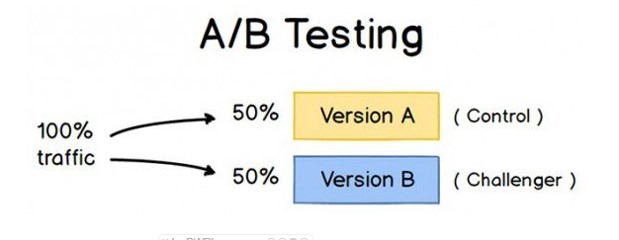
\includegraphics[scale=0.7]{abtest.jpg}
\caption{Process of A/B test Algorithm}
\end{figure}
\textbf {Steps in A/B testing algorithm}:-
\newline
\begin{enumerate}
\item For every user visiting the form, a form out of all the forms to choose is shown randomly.
\item When user submits a particular form, corresponding form score is updated.
\item When new user comes, go to step 1.
\item At the end of the testing period, each form's performance is compared and best form is decided. 
\end{enumerate}
\subsubsection{Adaptive Epsilon Greedy test Algorithm}
\begin{enumerate}
\item Set explore min count=0, X=initial epsilon value, N= no. of people to test, T=0 (no. of people submitted the form at a situation)
\item For every user visiting the form, check if explore min count equals M. If yes, set explore min count equals 0 and go to step 3 else go to step 4.
\item Calculate new epsilon value.
\item Select epsilon value from database and check for exploration or exploitation. Go to step 5.
\item If its explore, then show random form to user else show best form to user.
\item If user submits the form, then collect user characteristics and store details in the database. Update the performance of form and statistics in the database.
\item If T== N, then go to step 8, else go to step 2.
\item Stop running the algorithm and always show the best form which is decided by the performance in the test.
\end{enumerate}
\begin{figure}[H]
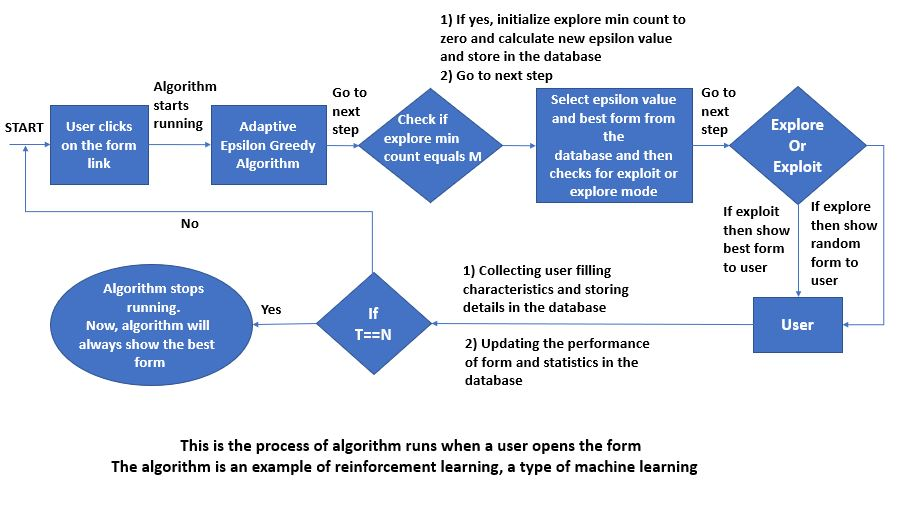
\includegraphics[scale=0.7]{flowchart.jpg}
\caption{Process of Adaptive Epsilon Greedy Algorithm}
\end{figure}
\textbf{Explore min count (between 0 and M) } = The count which tells the no. of explorations done and  initialized to 0 after M explorations.
\newline \textbf{M} = The no. of explorations after which the best form has to be selected and epsilon value to be adjusted.
\newline \textbf{T} = The user no. of last user who filled the form.
\newline \textbf{N} = The no. of users for which the test has to be conducted.

\chapter{Implementation detials}
The different versions of form has to integrated with Adaptive Epsilon Greedy Algorithm. An initial epsilon value has to be set. As the algorithm starts running, the epsilon value adjusts automatically (increases or decreases) according to the responses given by the user. 
For eg:- If the epsilon value is 0.1, then exploration will be done 10\% of the time and exploitation will be done 90\% of the time. And suppose, if the performance in the exploration phase will be good, then epsilon value increases depending on the percentage increase or decrease in the performance of the exploration phase. The epsilon value cannot become greater than 0.5.The test should be done for the number of users specified by the website owner. However, the more the versions of forms, the more the users should be considered. The more the number of users, the accurate will be the results.
\newline
After the end of experiment, the best form will be the one which has maximum score. The owner can also see the performance of the form on the dashboard. The performance of forms is shown in the form of curve. If the owner of website is not satisfied with the results, he can still continue the test with some set of users.
\newline
\newline
The questions asked in form are based on personal information. Question asked in the form are given below.
\begin{enumerate}
\item What is your first name?
\item What is your middle name?
\item What is your surname?
\item What is your age category?
\item What are your hobbies?
\item Have you participated in any social service camp? If yes, what is it?
\item What is your favourite sport?
\item What is your favourite TV show?
Which food item do you like?
\end{enumerate}
There were three forms called form 1, form 2 and form 3.
\newline
Form 1 contains question numbers 1 2 3 4 5 6 7 8 9
\newline
Form 2 contains question numbers 1 2 3 4 5 6 9
\newline
Form 3 contains question numbers 1 2 3 4 5 6
\newline
\section{A/B test table fields}
The table for A/B tests stores the following information apart from the fields
\newline

\begin{tabular}{ |p{3cm}|p{12cm}|  }
\hline
\multicolumn{2}{|c|}{\textbf {A/B test table details}} \\
\hline
\textbf { Column} & \textbf { Definition}  \\
\hline
user no & The serial no. of user who fills the form. It has autoincrement property.  \\
\hline
version no & The version of form.    \\
\hline
hash & Hash value is used to recognize the user properly at the server side.  \\
\hline
Filled  &  If the user submits the form, then it contains “yes” else “no”. \\
\hline
Score & Score assigned to form out of 2.  \\
\hline
no\_filled & The no of fields filled by the user \\
\hline
no\_of\_Fields & The no. of fields in the form.  \\
\hline
created at & It contains date time value at which the record is inserted.  \\
\hline
Percentage & Percentage of number of fields filled by the user out of total fields   \\
\hline
fill time & Time taken to fill the form.  \\
\hline
\end{tabular}
\newpage
\section{Adaptive Epsilon Greedy  tables}
\subsection{ Epsilon Greedy form fields}
There are two tables for Epsilon Greedy Algorithm.
\newline
The first table stores the user filled info.
\newline
\newline
\newline
\begin{tabular}{ |p{3cm}|p{12cm}|  }
\hline
\multicolumn{2}{|c|}{ \textbf {Epsilon Greedy test table details}} \\
\hline
 \textbf {Column} & \textbf { Definition}  \\
\hline
user no & The serial no. of user who fills the form. It has autoincrement property.  \\
\hline
Experiment & The experiment which is being performed (Explore/Exploit)  \\
\hline
version no & The version of form. It can be 1, 2 or 3.   \\
\hline
hash & Hash value is used to recognize the user properly at the server side.  \\
\hline
Filled  &  If the user submits the form, then it contains “yes” else “no”. \\
\hline
Score & Score assigned to form out of 2.  \\
\hline
no\_filled & The no of fields filled by the user \\
\hline
no\_of\_Fields & The no. of fields in the form.  \\
\hline
created at & It contains date time value at which the record is inserted.  \\
\hline
Percentage & Percentage of number of fields filled by the user out of total fields   \\
\hline
fill time & Time taken to fill the form.  \\
\hline
\end{tabular}
\newpage
\subsection { Performance fields of Epsilon Greedy}
The second table contains the performance parameters of each form and also the fields used to calculate the performance paramters.
\newline
\begin{tabular}{ |p{3cm}|p{12cm}|  }
\hline
\multicolumn{2}{|c|}{\textbf {Epsilon Greedy test performance table details}} \\
\hline
\textbf { Column} & \textbf {Definition}  \\
\hline
Exploit  & The no. of times exploitation done till the current user.  \\
\hline
Explore & The no. of times exploration done till the current user.  \\
\hline
Total & The sum of exploration and exploitation.   \\
\hline
M & It tells how many times to perform the exploration mode before the adaptive action which changes the value of Epsilon.  \\
\hline
Explore min count  &  It tells how many times exploration mode has been performed after the adaptive action which changes the value of Epsilon. \\
\hline
Previous explore percentage & The exploration percentage at which Explore min count becomes 0.  \\
\hline
Current explore percentage &The current exploration percentage. When explore min count equals 0, then current explore percentage is assigned to previous explore percentage. \\
\hline
Epsilon & The value of epsilon which decides the percentage of exploration and exploitation to be done.  \\
\hline
Form 1 &It gives the average score of form 1 ( form1 score/form1 count)	.  \\
\hline
Form 2 &It gives the average score of form 2 ( form2 score/form2 count)	   \\
\hline
Form 3 & It gives the average score of form 3 ( form3 score/form3 count)  \\
\hline
X & The initial epsilon value.  \\
\hline
Form 1 score & The sum of all the scores earned by form 1 till the current user.  \\
\hline
Form 2 score & The sum of all the scores earned by form 2 till the current user.  \\
\hline
Form 3 score &The sum of all the scores earned by form 3 till the current user.\\
\hline
Best & The best form at the current situation.  \\
\hline
Explore score & The sum of all the scores scored in the exploration mode.)  \\
\hline

\end{tabular}

\chapter{Results}
\begin{itemize}
\item	We made a dashboard for admin to check performance of each form. The results consists of exploration percentages of A/B test and Adaptive Epsilon Greedy test as well as the performance of each form of both the tests.
\item	For the performance graph of both algorithms,
\item	The X-axis defines the no. of users and Y- axis defines the formula of each form.
\item	The formula is given as

\item	Performance of form i after n users filling the form (i=form number) is given as\newline
Performance = (Cumulative score of a form i till the nth user)/(2*n)
\end{itemize}
\section{ A/B test}

\subsection{Exploration percentage}
\begin{figure}[H]
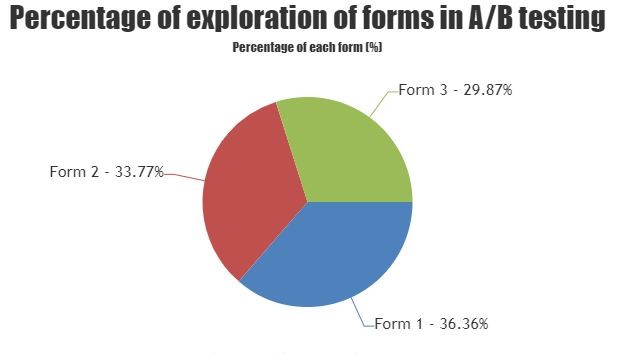
\includegraphics[scale=1]{abtestpie.jpg}
\caption{Exploration percentage of each form in A/B testing}
\end{figure}
\begin{itemize}
\item	In the case of A/B testing, each form gets approximately equal chances for exploration.
\item	As per the above Pie chart, Form 1, Form 2 and Form 3 are explored for 36.36\%, 33.77\%, 29.87\% respectfully.
\item	So, by seeing the percentages, it seems that each form is approximately equally explored.
\end{itemize}
\subsection{Performance of each form}
\begin{figure}[H]
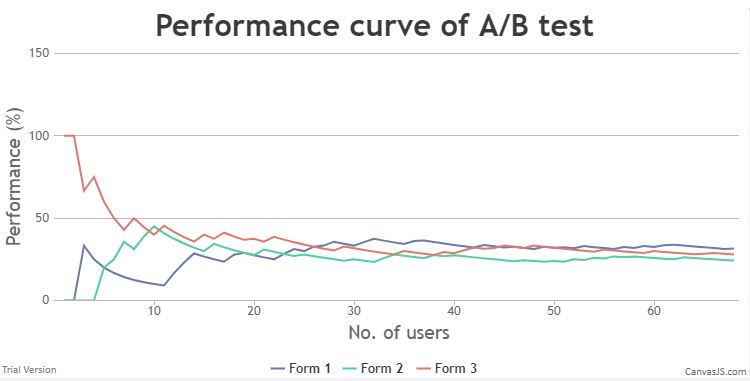
\includegraphics[scale=0.8]{performanceabtest.jpg}
\caption{Performance of each form in A/B testing}
\end{figure}

\begin{itemize}
\item From the above graph, we can see that performance of form 1 is better than the other two forms and it has become constant later. So, we can conclude that form 1 is the best form.
\item As we see in performance chart, form 2 and form 3 was not performing well, we still explored for 33.77\% and 28.87\% respectfully as given in the pie chart
\item So, during exploration using A/B testing we didn’t earn anything and we lose conversions.
\end{itemize}
\newpage

\section{Adaptive Epsilon Greedy Test}
\subsection{Exploration percentage}
\begin{figure}[H]
\caption{Exploration percentage of each form in Adaptive Epsilon Greedy Testing}
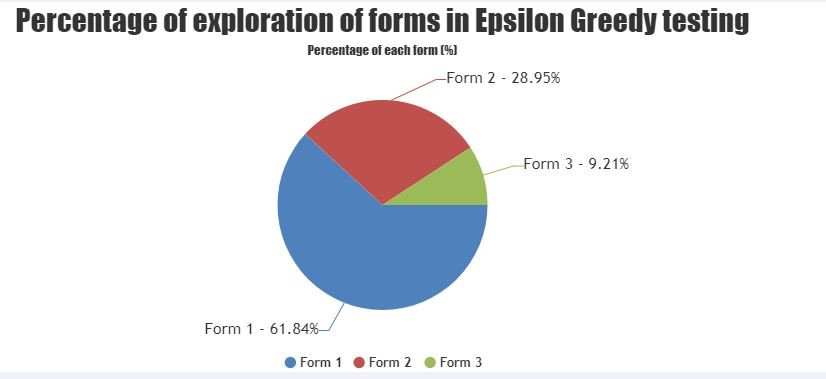
\includegraphics[scale=0.8]{epsilonpie.jpg}
\end{figure}
\begin{itemize}
\item In the case of the Adaptive Epsilon Greedy Algorithm, exploration of the forms is done as per epsilon value.
\item As per the above Pie chart, Form 1, Form 2 and Form 3 are explored for 61.84\%, 28.95\%, 9.21\% respectfully.
\end{itemize}

\subsection{Performance of each form}
\begin{figure}[H]
\caption{Performance of each form in Adaptive Epsilon Greedy Testing}
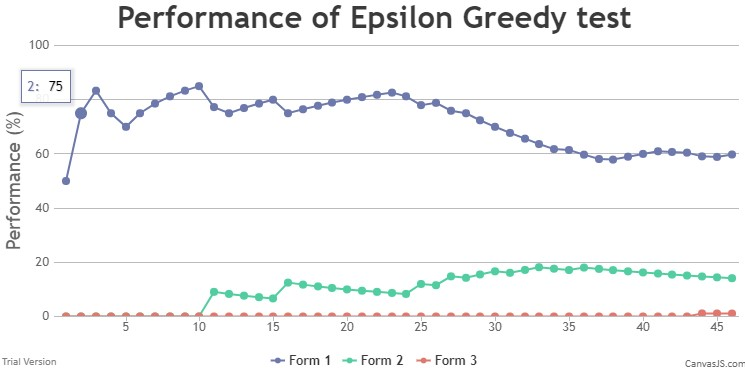
\includegraphics[scale=0.8]{performanceepsilon.jpg}
\end{figure}
\begin{itemize}
\item From the above graph, we can see that performance of form 1 is better than other two forms.
\item Hence, form 2 and form 3 has been explored less due to their poor performance which algorithm came to know at the beginning.
\item So, exploration for Form 2 and Form 3 is reduced to 28.95\% and 9.21\% respectfully.
\item But still it gave chance to form 2 and form 3 sometimes by expecting that it may perform well in the future. The algorithm’s behaviour changes according to the situation. This does not happen in A/B test. A/B test behaviour is same every time no matter which version performs well.
\item Hence, we are not losing conversions in Adaptive Epsilon Greedy as we lose in A/B test.
\end{itemize}
\chapter {Conclusion}
\section{Applications}
 An organization can predict the future performance of the form without losing customers. ‌An organization can increase their revenue. This algorithm can be implemented in websites having sign up forms, feedback forms and also social media sites.This project helps organization and developer to make web form very efficient and to get needed information from users by taking implicit feedback.


\section{Future enhancements}
We have implemented our algorithm for Web form. It can be implemented for other elements of website like logo, background color, navigation bar etc. This algorithm can be extended for entire web page or web site.

\section{Final conclusion}
Using the modern technology web stack, we have built a system which will be able to find the best form in an efficient way. We have performed A/B test and Adaptive epsilon greedy test for forms of three versions with a set of users and found out that Adaptive epsilon greedy algorithm finds the best form quickly and efficiently than A/B test. The fields we used in the form were based on personal information.This algorithm will help us to save lot of time and resources while exploring. Thus project on web form optimization using machine learning has been successfully implemented.
\newpage
\bibliographystyle{plainnat}
\bibliography{References}
\vspace*{40px}
\end{document}